%!TEX program = xelatex
\documentclass[tikz, border=3mm]{standalone}
\usepackage{pgfplots}
\usepackage{xcolor}
\usepgfplotslibrary{colormaps}
\pgfplotsset{
    compat=1.18,
    trig format plots=rad,  % 启用弧度制
    colormap/spring
}

\begin{document}
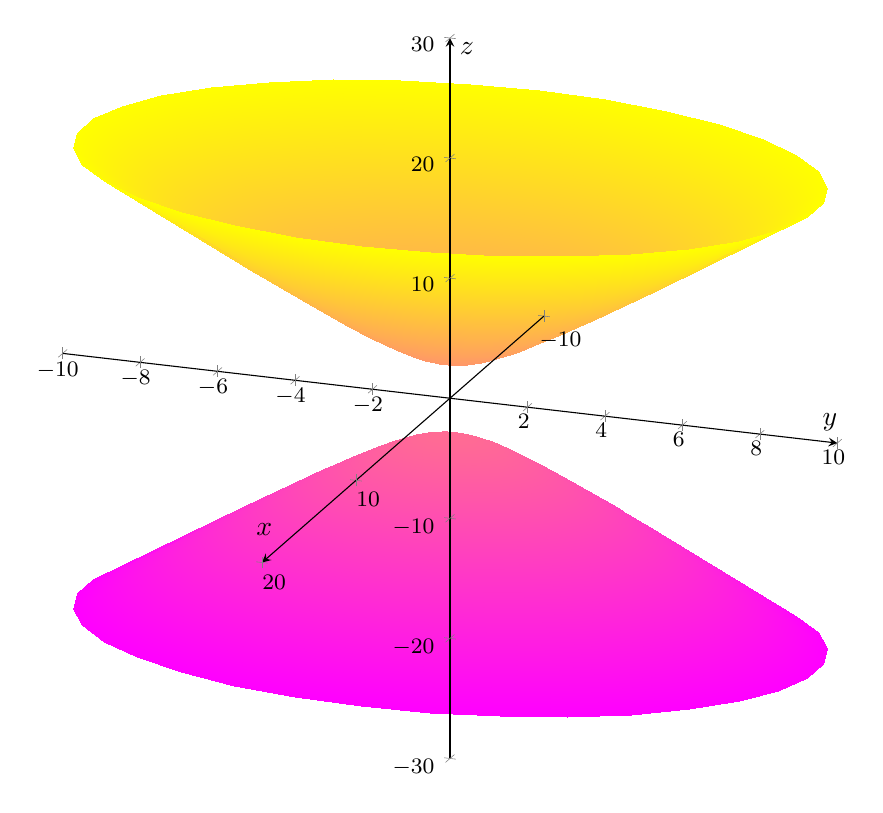
\begin{tikzpicture}
    \begin{axis}[
        view={110}{20},
        axis lines=center,
        xlabel=$x$, ylabel=$y$, zlabel=$z$,
        xmax=20, xmin=-10,
        ymax=10, ymin=-10,
        zmax=30, zmin=-30,
        width=15cm,           % 优化显示尺寸
        height=15cm,
        tick label style={font=\footnotesize},
        axis on top,
        clip=false            % 防止曲面被裁剪
    ]
        % 上半曲面
        \addplot3 [
            surf,
            z buffer=sort,
            samples=25,       % 优化采样率
            samples y=35,
            domain=0.55*pi:1.4*pi,
            y domain=0:2*pi,
            shader=interp
        ] (
            {1.5*tan(x)*cos(y)},
            {1.5*tan(x)*sin(y)},
            {3*sec(x)}
        );
        
        % 下半曲面
        \addplot3 [
            surf,
            z buffer=sort,
            samples=25,
            samples y=35,
            domain=0.55*pi:1.4*pi,
            y domain=0:2*pi,
            shader=interp
        ] (
            {1.5*tan(x)*cos(y)},
            {1.5*tan(x)*sin(y)},
            {-3*sec(x)}
        );
    \end{axis}
\end{tikzpicture}
\end{document}